% Full instructions available at:
% https://github.com/elauksap/focus-beamertheme

\documentclass{beamer}
\usetheme{focus}

\usepackage{wrapfig}
\usepackage{csquotes}
\usepackage{listings}
\usepackage{verbatim}
\usepackage{hyperref}
\usepackage{graphicx}
\usepackage{xparse}

\AtBeginSection[]
{
  \begin{frame}
    \frametitle{Table of Contents}
    \tableofcontents[currentsection]
  \end{frame}
}

\title{Using LaTeX and Markdown for Reproducible Research}
\subtitle{}
\author{Erik Beck \\ Emily Y. Li}
\titlegraphic{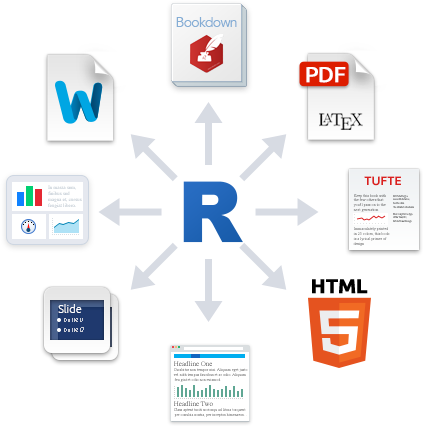
\includegraphics[width = 4.75cm]{Rlogotree.png}}
\institute{2018 US EPA \\ R User Group Workshop}
\date{11 Sept 2018}

\begin{document}
    \begin{frame}
        \maketitle
    \end{frame}
    
    \begin{frame}
        \frametitle{Table of Contents}
        \tableofcontents
    \end{frame}

\section{Agenda}

\begin{frame}{Time Frame \& Objectives}
\begin{exampleblock}{Using LaTeX and Markdown for Reproducible Research}
\begin{center}
    \begin{tabular}{c c c}
    Day & Time & Room \\
    \textbf{Tues, Sept 11} & \textbf{8:30-11:30am} & \textbf{C111C}
\end{tabular}
\end{center}
\end{exampleblock}

\begin{itemize}
    \item This 1/2-day workshop will provide attendees with hands-on experience
using the basics of LaTeX, Markdown, and the R package knitr.
    \item After attending this workshop, you will be able to use these tools to
facilitate reproducible reports and research with R.
\end{itemize}
% This would be a really good place to check that everyone has R and RStudio installed.
\end{frame}

\begin{frame}{Steps/Agenda}
We will try to use our three hours as effectively as possible.

\begin{exampleblock}{Rough Agenda}
%\begin{description}
%\item[8:30] System checks
%\item[8:45] Intro to LaTeX
%\item[9:00] Intro to Markdown
%\item[9:15] Markdown \& LaTeX
%\item[9:40] Reproducible Research
%\hline
%\item[9:50] \emph{BREAK}
%\hline
%\item[10:00] Dynamic documents with Sweave and knitr
%\item[10:30] Markdown \& LaTeX with R
%\end{description}
\begin{center}
\begin{tabular}{r|r|l}
    \textbf{\#} & \textbf{Time} & \textbf{Topic} \\
    1 & 8:30 & System checks \& agenda \\
    2 & 8:45 & Intro to LaTeX \\
    3 & 9:00 & Intro to Markdown \\
    4 & 9:15 & Markdown \& LaTeX \\
    5 & 9:40 & Reproducible Research \\
    \hline
     & 9:50 & \emph{BREAK} \\
    \hline
    6 & 10:00 & Dynamic documents with Sweave and knitr \\
    7 & 10:30 & Markdown \& LaTeX with R \\
    8 & 11:20 & Wrap-up \& additional resources
\end{tabular}
\end{center}
\end{exampleblock}
% We definitely want to go over these times before the workshop!
\end{frame}

\section{Introduction to LaTeX}
\begin{frame}{Intro to LaTeX}
LaTeX is a tool for high-quality typesetting based on the idea that it is better to leave document design to document designers, and to let authors get on with writing documents.
\vfill
\begin{block}{How do you pronounce ``LaTeX''?}
    \begin{quote}
        TeX is usually pronounced tech, making \emph{'lah}-teck, lah-\emph{'teck}, and \emph{'lay}-teck the logical choices; but language is not always logical, so \emph{'lay}-\emph{'tecks} is also possible.
    \end{quote}
    --- Leslie B. Lamport, original developer of \LaTeX{}
\end{block}
\end{frame}

\begin{frame}{Intro to LaTeX}
LaTeX is widely used in academia for the publication of scientific documents in many fields, including mathematics, statistics, computer science, engineering, chemistry, physics, economics, and political science.

\begin{enumerate}
    \item \textbf{TeX engines have excellent quality output.} This especially holds for complex documents such as those with mathematics, with many tables, or many cross-references or hyperlinks, or just with many pages.
    \item \textbf{TeX is fast.}
    \item \textbf{TeX is stable.} It will never eat your document. \emph{Ever.}
\end{enumerate}
\vfill
--- \url{https://www.ctan.org/tex/}
\end{frame}

\begin{frame}[fragile]{LaTeX: Minimal example}
Here is a minimal example of a full document written in LaTeX.
\begin{exampleblock}{}
\begin{lstlisting}
\documentclass{article}
\title{A Minimal LaTeX Example}
\author{Emily Li}

\begin{document}
\maketitle

Hello world!

\end{document}
\end{lstlisting}
\end{exampleblock}
% We will revisit this code later to make sure everyone compiled it.
\end{frame}

\begin{frame}{Levels of LaTeX: A disambiguation}
\begin{alertblock}{Help! There are too many words with ``TeX'' in them!}
If you are wondering, \alert{\emph{``Should I use LaTeX or MiKTeX?''}}, allow us to clear that up. These two slides will cover four types of TeX-related terms: distributions, editors, engines, and formats.
\end{alertblock}
\begin{enumerate}
    \item \textbf{Distributions:} \textit{MiKTeX, TeX Live, etc.} This is TeX-related software to be downloaded and installed. When someone says, ``I need to install TeX on my machine,'' they're usually looking for a distribution.
    \item \textbf{Editors:} \textit{Emacs, TeXworks, TeXShop, TeXStudio, etc.} These editors are what you use to create a document file. Some (e.g., TeXShop) are devoted specifically to TeX, while others (e.g., Emacs) can be used to edit any sort of file.
\end{enumerate}
\vfill
--- \url{http://www.tug.org/levels.html}
\end{frame}
\begin{frame}{Levels of LaTeX: A disambiguation}
\begin{exampleblock}{A quick note on editors}
You can also use Notepad to edit plaintext, including LaTeX code.
\end{exampleblock}
\begin{enumerate}
\setcounter{enumi}{2}
    \item \textbf{Engines:} \textit{TeX, pdfTeX, XeTeX, LuaTeX, etc.} These are the executable binaries which implement different TeX variants. When someone says, ``TeX can't find my fonts,'' they usually mean an engine.
    \item \textbf{Formats:} \textit{LaTeX, plain TeX, etc.} These are the TeX-based languages in which one actually writes documents. When someone says, ``TeX is giving me a mysterious error,'' they usually mean a format. (Incidentally, ``LaTeX'' has meant ``LaTeX2e'' for many years now.)
\end{enumerate}
\vfill
--- \url{http://www.tug.org/levels.html}
\end{frame}

\begin{frame}{LaTeX Distributions}
To compile LaTeX, your computer needs one of these TeX distributions installed:
\begin{block}{TeX Distributions}
\begin{center}
    \begin{tabular}{c l}
    Distribution & Operating System \\
    \hline
    MiKTeX & Windows OS \\
    TeX Live & Linux and other UNIX-like systems \\
    MacTeX & Mac OS X
\end{tabular}
\end{center}
\end{block}
You can also use an on-line, ready-to-use option like \href{https://www.sharelatex.com/}{ShareLaTeX} or \href{https://www.overleaf.com/}{Overleaf}.
\end{frame}

\begin{frame}[fragile]{LaTeX: Revisiting the minimal example}
\begin{exampleblock}{Try compiling this LaTeX}
\begin{lstlisting}
\documentclass{article}
\title{A Minimal LaTeX Example}
\author{Emily Li}

\begin{document}
\maketitle

Hello world!

\end{document}
\end{lstlisting}
\end{exampleblock}
\end{frame}

\section{Introduction to Markdown}
\begin{frame}{Intro to Markdown}
\begin{columns}[t, onlytextwidth]

\column{0.5\textwidth}
\vfill
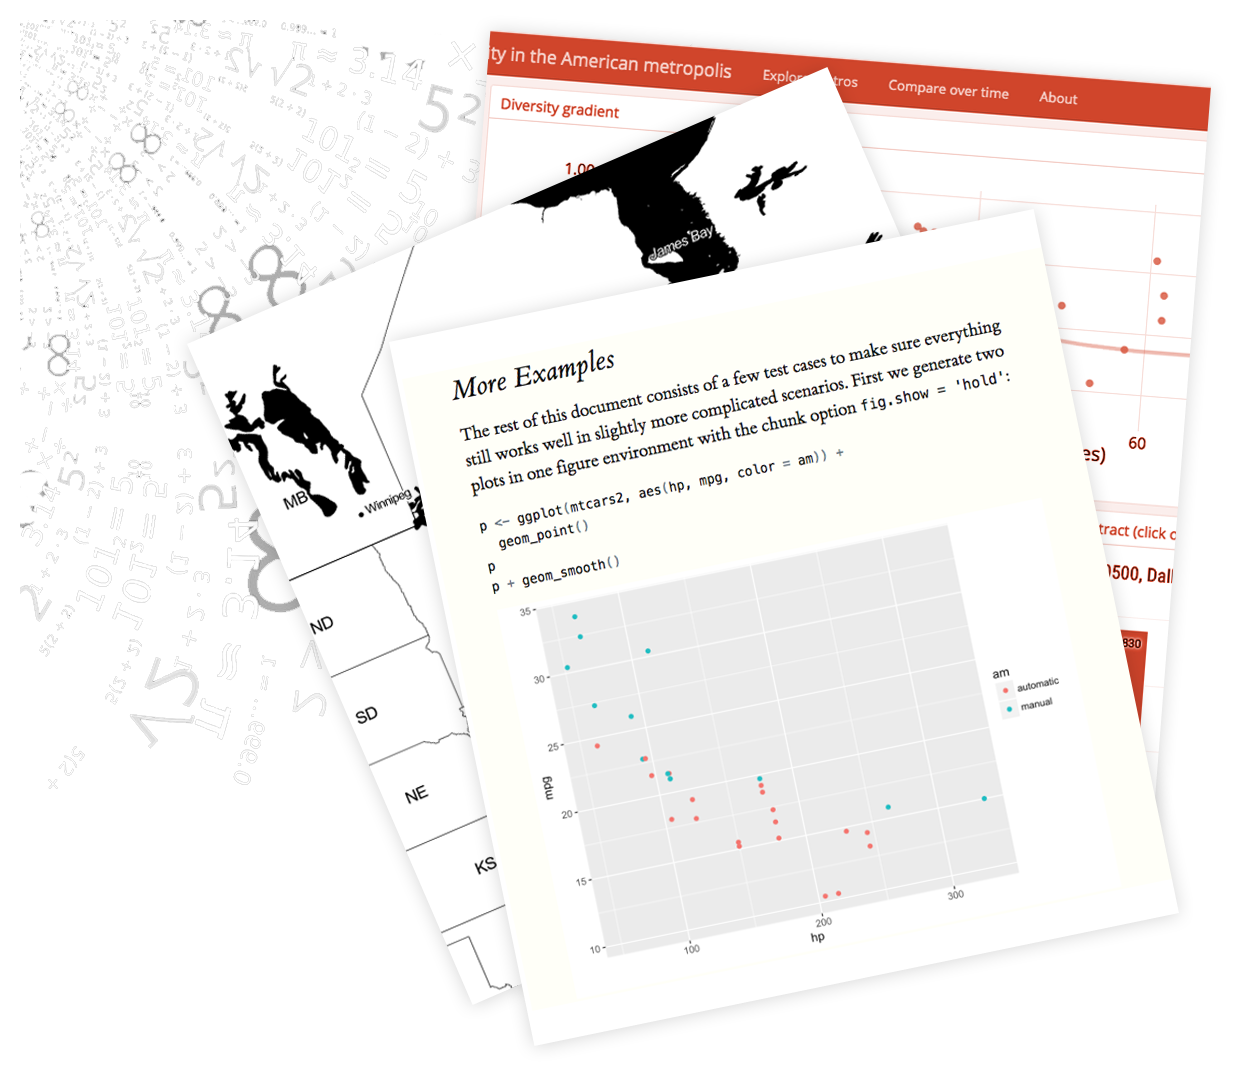
\includegraphics[width=\textwidth]{markdown-examples.png}
\vfill
{\footnotesize \url{https://rmarkdown.rstudio.com/}}

\column{0.5\textwidth}
    \begin{itemize}
        \item An \textbf{.Rmd file} is an R Markdown file
        \item Contains the code that a scientist needs to reproduce your work, along with the narration that a reader needs to understand your work.
        \item Choose to export the finished report in a variety of formats, including HTML, PDF, or MS Word.
    \end{itemize}

\end{columns}
\end{frame}

\begin{frame}{Intro to Markdown}
\begin{itemize}
    \item Markdown allows us to write using an easy-to-read, easy-to-write plain text format.
    \item As long as you know how to write emails, you can learn it in a few minutes.
    \item \url{https://en.wikipedia.org/wiki/Markdown#Example}
\end{itemize}
\vfill
\begin{alertblock}{Limitations of Markdown}
Markdown was primarily designed to be simple. \\ For more complicated typesetting, LaTeX may be preferred.
\end{alertblock}
\end{frame}

\begin{frame}[fragile]{Intro to Markdown}
\begin{exampleblock}{A short example of Markdown}
\begin{lstlisting}
# First level header

Hello world!

## Second level header

This is **bold**, and _italic_.
- list item
- list item

You can write an ordered list:
1. item 1
1. item 2 # this line will render as "2."
\end{lstlisting}
\end{exampleblock}
\end{frame}

\begin{frame}{Workflow in Markdown}
Using RStudio:
\begin{description}
\item[Open] a new .Rmd file, which pre-populates with a template
\item[Write] a document by editing the template
\item[Knit] the document to create a report; use the knitr button or render() to knit
\item[Preview] output in IDE window
\item[Publish] to web server (optional)
\item[Use] output file that is saved alongside .Rmd
\end{description}
\vfill
Helpful link: \\ \url{https://rmarkdown.rstudio.com/lesson-2.html}
\end{frame}

\section{Markdown \& LaTeX}


\section{Reproducible Research}
\begin{frame}[noframenumbering]{Reproducible Research}
\begin{center}
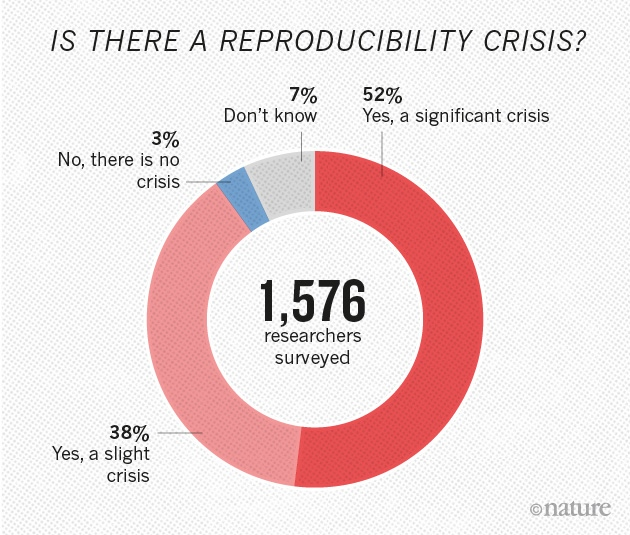
\includegraphics[width=.82\textwidth]{nature-reproducibility-graphic.jpeg}
\end{center}
\vspace{-0.5cm}
{\footnotesize \href{https://www.nature.com/news/1-500-scientists-lift-the-lid-on-reproducibility-1.19970}{\textit{Nature} \textbf{533}, 452-454 (26 May 2016) | doi:10.1038/533452a}}
\vfill
\end{frame}

\begin{frame}[noframenumbering]{Reproducible Research}
    \begin{center}
        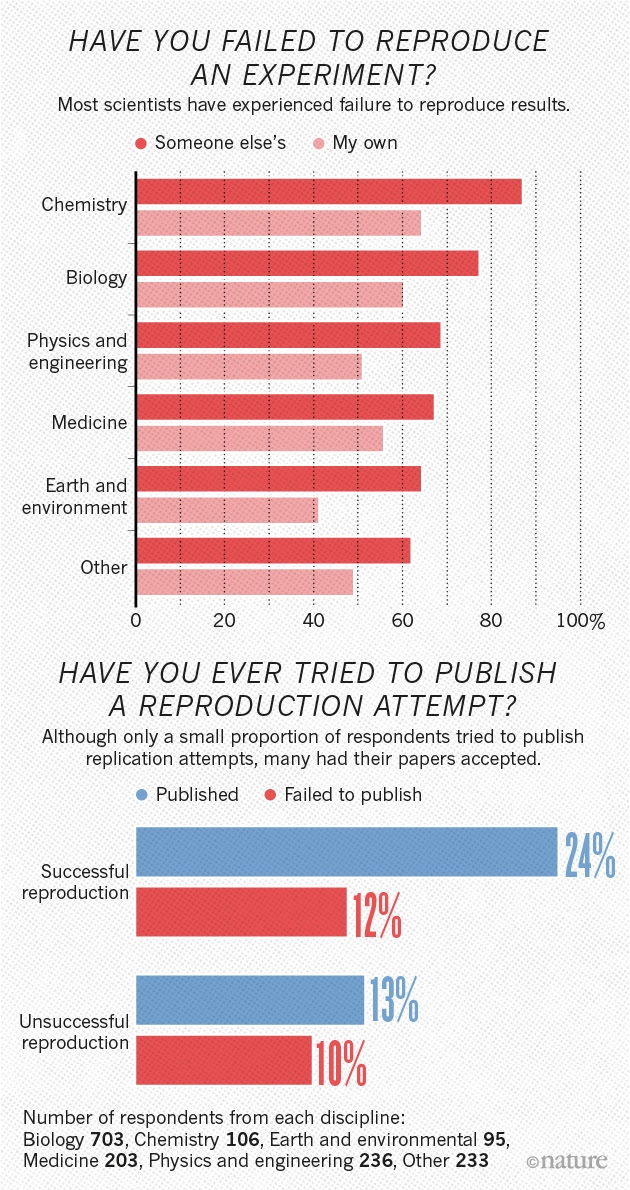
\includegraphics[trim=0 550 0 15, clip, width=.71\textwidth]{nature-reproducibility-breakdown.jpg}
    \end{center}
\vspace{-0.5cm}
{\footnotesize \href{https://www.nature.com/news/1-500-scientists-lift-the-lid-on-reproducibility-1.19970}{\textit{Nature} \textbf{533}, 452-454 (26 May 2016) | doi:10.1038/533452a}}
\vfill
\end{frame}

\begin{frame}{Reproducible Research}
\begin{alertblock}{Results must be reproducible to be trustworthy.}
\begin{quote}
    An article about computational science in a scientific publication is not the scholarship itself, it is merely the advertising of the scholarship. The actual scholarship is the complete software development environment \textbf{and the complete set of instructions which generated the figures}.
\end{quote}
\end{alertblock}
--- 1995, David L. Donoho, professor of statistics at Stanford University
\vfill
    % Though Donoho was referring to computational science, journals in other data-driven fields such as biostatistics have been moving in the direction of reproducible research as well.
    % This would be a good time to quickly discuss attendees' difficulties with reproducing research.
\end{frame}
    
\begin{frame}[fragile]{Reproducible Research}
This chunk of R code produces a figure that illustrates a simulation of Brownian motion for 100 steps.
        \begin{exampleblock}{Try running this in RStudio}
\begin{lstlisting}
set.seed(1213) # for reproducibility
x <- cumsum(rnorm(100))
plot(x, type = ''l'',
    ylab = ''$x_{i+1}=x_i+\\epsilon_{i+1}$'',
    xlab = ''step'')
\end{lstlisting}
        \end{exampleblock}
\end{frame}

\begin{frame}[fragile]{Reproducible Research}
        \begin{exampleblock}{}
\begin{lstlisting}
set.seed(1213)
x <- cumsum(rnorm(100))
plot(x, type = ''l'',
    ylab = ''$x_{i+1}=x_i+\\epsilon_{i+1}$'',
    xlab = ''step'')
\end{lstlisting}
        \end{exampleblock}
To put this into a document by hand, we would have to open RStudio, compile the code to draw the plot, save it as an image, then insert it into a document with \verb|\includegraphics{}| in LaTeX or 'Insert Image' in Word.
\vfill
Then what if we want to change the random seed in \verb|set.seed()|, or the y-axis label?
% This is both tedious and difficult for the author to maintain. If we want to change the figure, we have to update both the source code and the typesetting file.
\end{frame}


\begin{frame}{Dynamic report generation}
% This slide is too wordy and long.
\begin{itemize}
    \item Instead of separating results from computing, we can put everything in one document, including the computational steps and narratives.
    \item When we compile this document, the computer code will be executed, giving us the results directly.
    \item Dynamic report generation by integrating code with narratives is not only easier, but also closely related to reproducible research.
    \item It does not guarantee RR, but RR is one possible by-product of dynamic documents.
\end{itemize}
\end{frame}

\begin{frame}[focus]
    Break for 10 minutes
    
    \vfill
    
\includegraphics[trim=100 0 100 0, clip, width=\textwidth]{stretching-work.png}
    \vspace{-0.5cm}
    {\tiny Image source \url{https://getcubefit.com/}. Not an endorsement of the company.}
\end{frame}

\begin{frame}[focus]
    Welcome back!
\end{frame}

\section{Dynamic documents with Sweave and knitr}

\begin{frame}[fragile]{Sweave}
    Sweave has been a longstanding tool for dynamic documents since 2002.
    \begin{itemize}
        \item Deals with Rnw documents, combining the power of R with the production value of LaTeX to enable reproducible research
        \item Part of base R---in the \textbf{utils} package as the \verb|Sweave()| function
        \item Two ways to run Sweave:
        \begin{itemize}
            \item From your R session: \verb|Sweave("your_file.Rnw")|
            \item From the command line: \verb|R CMD Sweave your_file.Rnw|
        \end{itemize}
    \end{itemize}
    \vfill
    However...
    \begin{itemize}
        \item Development has plateaued in recent years
        \item Extensions based on core code are no longer sycnhronized with Sweave development, have become incompatible.
        \item LaTeX (to produce Rnw documents) is more complicated than RMarkdown (Rmd), and documents rarely need to be produced as PDFs unless submitting a manuscript to journals.
    \end{itemize}
\end{frame}

\begin{frame}{knitr}
knitr was largely motivated by Sweave
First of all, knitr uses Rmarkdown, a set of intuitive human-readable code to do the formatting. While LaTeX is by no means as complicated as its reputation seems to suggest, Rmarkdown is actually easy. By human-readable I mean that anyone who has never even heard of Rmarkdown can understand what is happening to some extent.
Sweave is great for producing PDF, but that’s one of the biggest drawbacks of LaTeX in the social sciences: while the PDF may look good, they are not the format we need when collaborating with Word-only colleagues, and with rare exceptions when submitting a manuscript to journals. Knitr works very well with Pandoc, so creating a Word document or an ODF is just as easy as creating a PDF. The other day I had to submit a supplementary file as a *.doc file, even though it’ll end up as a PDF on Dataverse or so. With knitr this didn’t take long.
\end{frame}

\begin{frame}{Why knitr beats Sweave}
    \begin{itemize}
        \item 
    \end{itemize}
\end{frame}

\section{Markdown \& LaTeX with R}

\begin{frame}{Markdown \& LaTeX side-by-side}
    \begin{alertblock}{Apples \& Oranges?}
    The next few slides will show a side-by-side comparison of Markdown and LaTeX using the exact same analysis.
    \end{alertblock}
\end{frame}

\begin{frame}[fragile]{Example LaTeX with analysis}
\begin{lstlisting}
\documentclass{article}
\begin{document}
\title{Speed and Stopping Distance}
\author{Yihui Xie, creator of knitr}

\maketitle

We examine the relationship between speed and stopping distance using a linear regression model:
$Y = \beta_0 + \beta_1 x + \epsilon$.

<<model, fig.width=4, fig.height=3, fig.align='center'>>=
par(mar = c(4, 4, 1, 1), mgp = c(2, 1, 0), cex = 0.8)
plot(cars, pch = 20, col = 'darkgray')
fit <- lm(dist ~ speed, data = cars)
abline(fit, lwd = 2)
@

The slope of a simple linear regression is \Sexpr{coef(fit)[2]}.

\end{document}
\end{lstlisting}
% This LaTeX code does not seem to work in ShareLaTeX.
\end{frame}

\begin{frame}{R in LaTeX}
    When embedding R code in LaTeX, start a code chunk with <<>>= and terminate it with @.
\end{frame}

\begin{frame}[fragile]{Example Markdown with analysis}
\begin{lstlisting}
---
title: Speed and Stopping Distance
---

We examine the relationship between speed and stopping distance using a linear regression model:
$Y = \beta_0 + \beta_1 x + \epsilon$.

```{r fig.width=4, fig.height=3, fig.align='center'}
par(mar = c(4, 4, 1, 1), mgp = c(2, 1, 0), cex = 0.8)
plot(cars, pch = 20, col = 'darkgray')
fit <- lm(dist ~ speed, data = cars)
abline(fit, lwd = 2)

The slope of a simple linear regression is `r coef(fit)[2]`.
\end{lstlisting}
% This Markdown code seems to work in RStudio.
\end{frame}

\begin{frame}{R in Markdown}
\begin{itemize}
    \item Quickly insert chunks with the keyboard shortcut Ctrl + Alt + I (OS X: Cmd + Option + I).
    \item By comparison, Markdown has simpler commands.
\end{itemize}
\end{frame}

\begin{frame}[fragile]{Markdown}
    \begin{itemize}
        \item Write code chunks between \verb|```{r}| and \verb|```|
        \item Inline R code is written in \verb|` `|
        \item Chunk options are written before closing brace in the chunk header.
    \end{itemize}
\end{frame}

\begin{frame}[fragile]{Quick reporting in Markdown}
    It is also possible to generate a quick report from R script using knitr's \verb|stitch()| function.
    \begin{exampleblock}{Usage of \verb|stitch()| for quick reports}
    \begin{lstlisting}
    library(knitr)
    stitch("your-script.R")
    \end{lstlisting}
    \end{exampleblock}
    \begin{itemize}
        \item \verb|stitch()| provides a template so the user only feeds the template with one R script and knitr will compile the template to a report.
        \item Currently it has built-in templates for LaTeX, HTML, and Markdown.
    \end{itemize}
\end{frame}

%\begin{frame}{Markdown and LaTeX syntax summary}
%    \begin{block}{A syntax summary of R LaTeX and R Markdown document formats.}
%    \begin{tabular}{l|l|l|l}
%        Format & Start chunk & End chunk & Inline code \\
%        \hline
%        Rnw & <<*>>= & @ & \begin{lstlisting}\Sexpr{x}\end{lstlisting} \\
%        Rmd & ```{r *} & ``` & `r x`
%    \end{tabular}
%    \end{block}
%\end{frame}

%    \begin{frame}[plain]{Plain frame}
%        This is a frame with plain style and it is numbered.
%    \end{frame}
    
%    \begin{frame}[t]
%        This frame has an empty title and is aligned to top.
%    \end{frame}
    
%    \begin{frame}[noframenumbering]{No frame numbering}
%        This frame is not numbered and is citing reference \cite{knuth74}.
%    \end{frame}
    
%    \begin{frame}{Typesetting and Math}
%        The packages \texttt{inputenc} and \texttt{FiraSans}\footnote{\url{https://fonts.google.com/specimen/Fira+Sans}}\textsuperscript{,}\footnote{\url{http://mozilla.github.io/Fira/}} are used to properly set the main fonts.
%        \vfill
%        This theme provides styling commands to typeset \emph{emphasized}, \alert{alerted}, \textbf{bold}, \textcolor{example}{example text}, \dots
%        \vfill
%        \texttt{FiraSans} also provides support for mathematical symbols:
%        \begin{equation*}
%            e^{i\pi} + 1 = 0.
%        \end{equation*}
%    \end{frame}

%    \begin{frame}{Lists}
%        \begin{columns}[t, onlytextwidth]
%            \column{0.33\textwidth}
%                Items:
%                \begin{itemize}
%                    \item Item 1
%                    \begin{itemize}
%                        \item Subitem 1.1
%                        \item Subitem 1.2
%                    \end{itemize}
%                    \item Item 2
%                    \item Item 3
%                \end{itemize}
%            
%            \column{0.33\textwidth}
%                Enumerations:
%                \begin{enumerate}
%                    \item First
%                    \item Second
%                    \begin{enumerate}
%                        \item Sub-first
%                        \item Sub-second
%                    \end{enumerate}
%                    \item Third
%                \end{enumerate}
%            
%            \column{0.33\textwidth}
%                Descriptions:
%                \begin{description}
%                    \item[First] Yes.
%                    \item[Second] No.
%                \end{description}
%        \end{columns}
%    \end{frame}

\section{Additional Resources}
\begin{frame}{Resources}
        \begin{columns}[t, onlytextwidth] \column{.5\textwidth}
        \begin{center}
            Erik Beck \\ \href{mailto:beck.erik@epa.gov}{beck.erik@epa.gov}
        \end{center}
        \column{.5\textwidth}
        \begin{center}
            Emily Y. Li \\ \href{mailto:li.emily@epa.gov}{li.emily@epa.gov}
        \end{center}
        \end{columns}
\vfill
\begin{itemize}
    \item \url{https://www.rstudio.com/resources/cheatsheets/}
    \item \url{https://support.rstudio.com/hc/en-us/articles/200552056-Using-Sweave-and-knitr}
    \item knitr document source + output examples: \url{https://yihui.name/knitr/demos/}
    \item To Markdown or LaTeX, that is the question: \url{https://yihui.name/en/2013/10/markdown-or-latex/}
\end{itemize}
\end{frame}

\begin{frame}[focus]
    Thanks for coming!
\end{frame}

%    \appendix
%    \begin{frame}{References}
%        \nocite{*}
%        \bibliography{demo_bibliography}
%        \bibliographystyle{plain}
%    \end{frame}
    
%    \begin{frame}{Backup frame}
%        \usebeamercolor[fg]{normal text}
%        This is a backup frame, useful to include additional material for questions from the audience.
%        \vfill
%        The package \texttt{appendixnumberbeamer} is used not to number appendix frames.
%    \end{frame}

\end{document}
